\chapter{Background}
\label{cha:background}
%At the begging of each chapter, please introduce the motivation and high-level
%picture of the chapter. You also have to introduce sections in the
%chapter. 


\section{Electronic Voting}
   Electronic voting is a nightmare because of a minuscule possibility of 
   bug in software used in voting could lead to a disaster, possibly 
   inverting the results[swisspost]. Given that the cost of 
   electronic voting is 
   so high, we should totally refrain from it; however, on contrary
   it is gaining popularity. Some of the notable countries using some form
   of electronic voting are Estonia (probably the only success story), India,
   Australia, Canada and USA. 
    \begin{figure}[htb]
	\begin{center}
	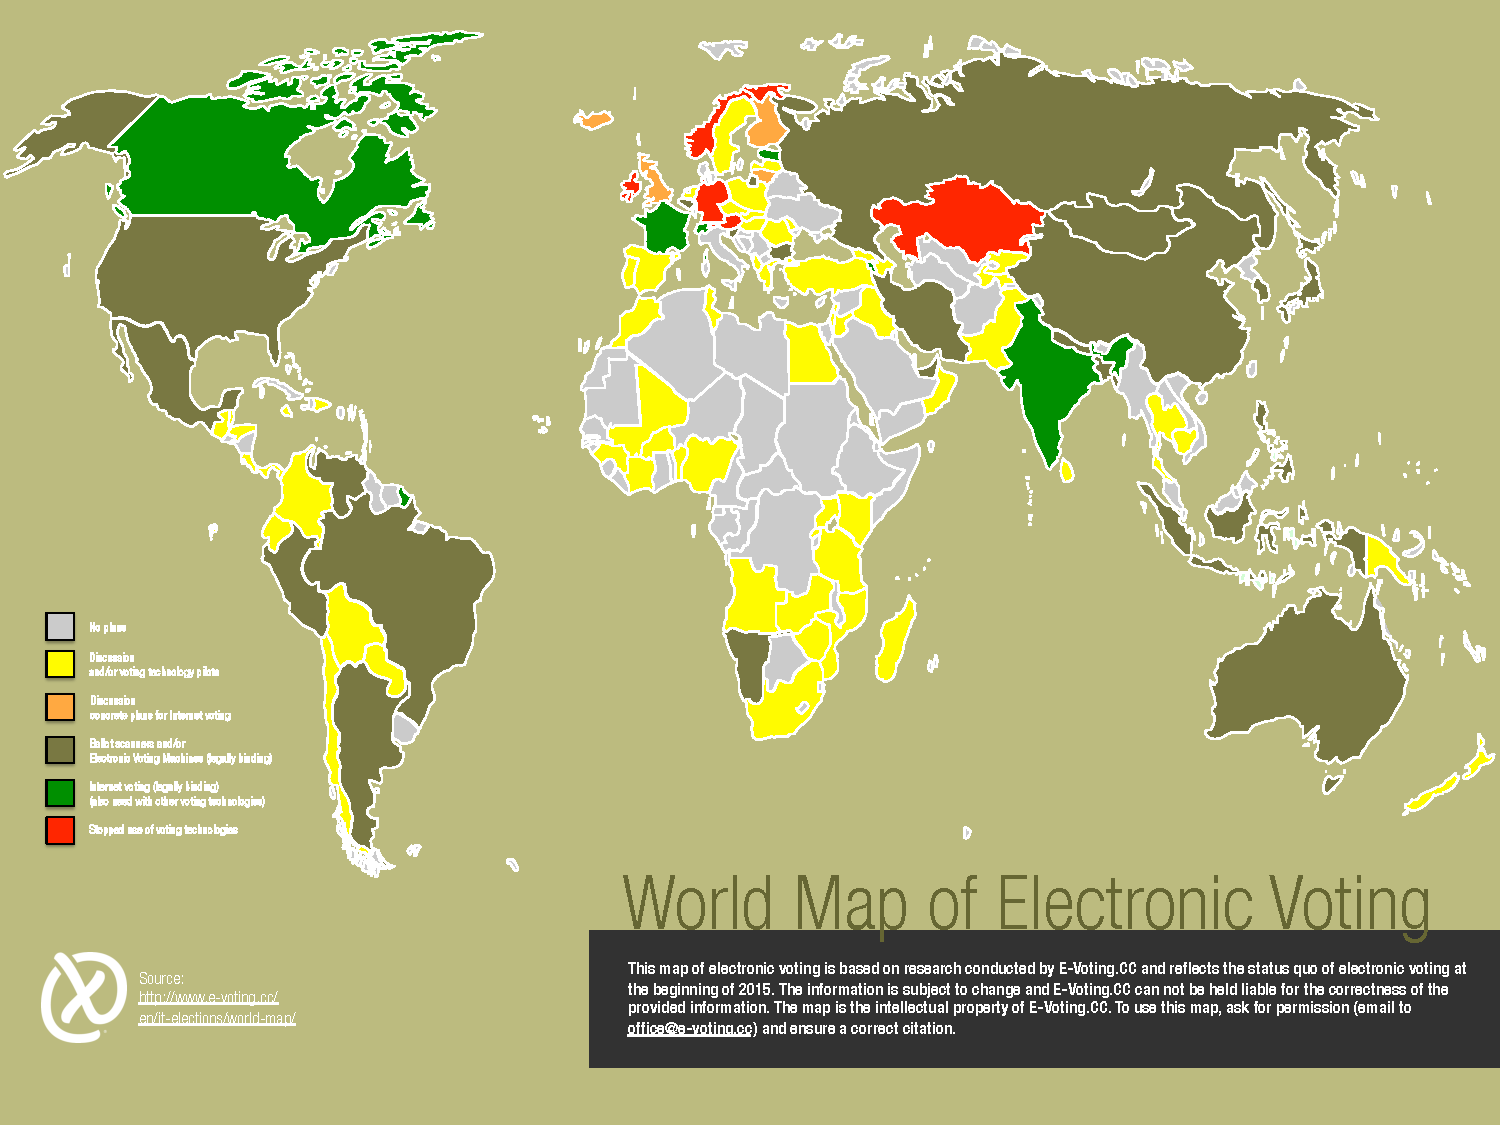
\includegraphics[scale=0.5]{e-voting_worldmap_2015.pdf}
	\caption{World map of Electronic Voting}
	\end{center}
  \end{figure}  
   
  The world can be divided into five categories on 
  parameter of electronic voting\footnote{https://www.e-voting.cc/en/it-elections/world-map}[Figure 2.1]
  \begin{itemize}
  \item No electronic voting (Grey Area)
  \item Discussion and/or voting technology pilots (Yellow Area)
  \item Discussion, concrete plans for Internet voting (Orange Area)
  \item Ballot scanners, Electronic Voting Machines, and Internet Voting
        (Green and Dark Green)
  \item Withdrawn voting technology because of public concern (Red Area)
        Germany, The Nederlands, and UK  
  \end{itemize}    
  
 

   
%  The input method, form of ballot, used the countries participating 
%  in electronic voting can be broadly divided into three group 
  Arguments in favour of electronic voting are 
  increased voter turnout, faster result and cost. Senate 
  election conducted in Western Australia in September 2013 were 
  declared void by high court because of loss of 1370 votes. It was 
  re-conducted in April 2014 with cost of 20 Million AUD with additional 
  delay in results\footnote{https://www.theguardian.com/world/2014/feb/28/western-australia-senate-election-re-run-to-be-held-on-5-april}. Sometimes, 
  the cost is not only concern, but the time involved in counting 
  is. \fix{Give a example of seat which took considerable amount 
  of time in declaring result}. 
  \fix{Add time and cost saving in Indian election after using 
  electronic voting machines} 
  The advantages of electronic voting 
  looks so promising, so why some countries (Red Area) retracted 
  from electronic voting ? Off course, electronic voting makes 
  the process faster, but it has its own layer of added complexities 
  which creates a trust issue among voters. 
  In 2005 German election, two voters filed a case in German 
  Constitutional Court (Bundesverfassungsgericht) because their 
  appeal to scrutinize the elections 
  was not heeded by the Committee. They argued that using electronic 
  voting machines to conduct the election was unconstitutional, and 
  these machines could be hacked, hence results of the 2005 election 
  could not be trusted. The case was argued on the grounds 
  of "all essential steps in the elections are subject to 
  public examinability." according to German Constitution 
  (Basic Law for the Federal Republic of Germany). 
  The Court noted that, under the constitution, elections are 
  required to be public in nature
  
  "The principle of the public nature of elections requires that all 
  essential steps in the elections are subject to public examinability
  unless other constitutional interests justify an exception. 
  Particular significance attaches here to the monitoring of the 
  election act and to the ascertainment of the election result. "
  \footnote{https://www.bundesverfassungsgericht.de/
  SharedDocs/Entscheidungen/EN/2009/03/cs20090303\_2bvc000307en.html}

  The court did not rule out or prevent the usage of electronic 
  voting machines,  but suggested to make the process more 
  transparent and trustworthy.  
  
  "The legislature is not prevented from using electronic voting machines 
  in the elections if the constitutionally required possibility of a 
  reliable correctness check is ensured. In particular, voting machines 
  are conceivable in which the votes are recorded elsewhere in addition
   to electronic storage. This is for instance possible with electronic
   voting machines which print out a visible paper report of the vote 
   cast for the respective voter, in addition to electronic recording 
   of the vote, which can be checked prior to the final ballot and is
    then collected to facilitate subsequent checking. Monitoring that is
     independent of the electronic vote record also remains possible when
     systems are deployed in which the voter marks a voting slip and the 
     election decision is recorded simultaneously, 
     or subsequently by electronic means in 
     order to evaluate these by electronic means at the end of the 
     election day."
  
  The Netherlands were among few countries who adopted electronic voting 
  in early nineties (1990), but it did not go very well long run and was 
  abolished in 2008 
  [http://www.cs.ru.nl/B.Jacobs/PAPERS/E-votingHistory.pdf]. 
  The reason for abolishing electronic voting was that   
  the voting machines used in election were susceptible to many attacks
   and could not stand 
  for public verifiability of results. The decision was victory for 
  Dutch public foundation, Wij vertrouwen stemcomputers niet
  \footnote{English Translation "We do not trust voting computers"}, which 
  demonstrated that e-voting machines used in election leaks enough
  information to guess the option, 
  and they can be easily intercepted from 20 to 30 meters
  \footnote{https://www.youtube.com/watch?v=B05wPomCjEY}. 
  
  
  Germany and The Netherlands are some of the rarest cases where 
  electronic voting was withdrawn because it was not able to 
  replicate the same trust environment as created by paper ballot.
  At this point, the reader can get into the impression that 
  countries who are using electronic voting have successfully 
  created the trust environment in electronic voting. Sadly, 
  it is not the case. India, one of the largest democracy in world, 
  uses electronic voting machines (also known as EVMs) for national 
  and state level 
  elections even though many political parties raised security 
  concern against it.
  It was already shown in 2010 in the paper 
  Security Analysis of India's Electronic Voting Machines by 
  Scott Wolchok et. al 
  [https://jhalderm.com/pub/papers/evm-ccs10.pdf] that it 
  is possible to manipulate the election results by replacing the 
  parts of machine with malicious look alike components with sending 
  them instructions over wireless
  \footnote{https://www.youtube.com/watch?v=ZlCOj1dElDY} 
  \footnote{https://indiaevm.org/}. 
  In recent elections of 2019, the Election Commission of India 
  announced, to ensure the transparency and 
  increase the trust of public, that it would use 
  voter-verified paper audit trail (VVPAT) 
  one per assembly; however, the Supreme Court of India ordered Election 
  Commission of India to increase it to five
  \footnote{https://www.news18.com/news/india/sc-directs-ec-to-increase-vvpat-verification-from-one-evm-to-five-evms-per-constituency-2093363.html}.
  The Commission  would count VVPAT slips 
  in randomly selected one polling booth per assembly 
  constituency in state election and 
  in one polling booth in each assembly segment for national election, but 
  now following the Supreme Court decision it has to do the same for 
  5 randomly selected assembly constituencies/segments. 
  \fix{Find out if there is a document at Election Commission of 
  India website and how the process works}. The design of these 
  machines are closely guard secret,  but it not impossible to gain 
  access as shown by  Scott Wolchok et. al. It would be more 
  interesting and beneficial for Indian democracy if Election 
  Commission of India
  releases the design to public scrutiny (very much like cryptographic
  implementation review process).
  
  
  
 
  
    
  
   
   \subsection{Software Bugs : Origin of Problem}
   
   
   \subsection{Estonia : Success Story}

   \subsection{Universal Verifiability}


\fix{Can I introduce Write Hilbert's idea of mathematical formalism/Frege}

A proof assistant is a computer program which assists users in development of mathematical proofs. The idea of 
developing mathematical proofs using computer goes back to Automath (automating mathematics)
[cite Automath] and LCF [cite Logic for computation] project. The 
Automath project (1967 until the early 80's)  was initiative of De Bruijn, and the aim of the project was to develop
a language for expressing mathematical theories which can be verified by aid of computer.  Automath was first 
practical project to exploit the Curry-Howard isomorphism (proofs-as-programs and formulas-as-types)
 [reference here]. DeBruijn  was likely unaware of this correspondence, and he almost re-invented it 
 ([Wiki entry on Curry-Howard]). Many researchers refers Curry-Howard isomorphism as 
 Curry-Howard-DeBruijn isomorphism. Automath project can be seen as the precursor of
 proof assistants NuPrl [cite here] and Coq [cite coq].   Some other notable  proof assistants are 
 LCF (Logic for Computable Functions)  [cite Milner?], Mizar [cite], Nqthm/ACl2 [cite], PVS [cite], 
 HOL (a family of tools derived from LCF theorem prover), Agda [cite], and Lean [cite].


In this chapter, I will give a overview of theoretical foundation of 
Coq thorem prover i.e. Calculus of Construction and  
Calculus of Inductive Construction, followed by Dependent type 
and how it leads to 
correct by construction (paradigm?) with a example of dependent 
typed lambda calculus. I will also discuss distinction between Type and Prop 
and how it affects the code extraction, a feature for extracting 
certified functional programs from specification proofs, and the 
specification language Gallina. Finally, I would 
argue that why should we trust the Coq proofs even though it does not 
match or look like a mathematical proof.



 
\section{Computer Programming and Type Theory}
	\begin{itemize}
	\item Some tracking of History about how type theory was introduced 
	     to computer programming. Use Dirk's expertise here
	\item Type theory is a logical foundation introduced by 
	      Russel to solve the problem of  paradox in Frege's 
	      Begriffsschrift.
	\item A Church invented formal system of computation, Lambda calculus
	\item A typed lambda calculus
	\item Curry Howard isomorphism
	\end{itemize}


\section{Coq: Interactive Theorem prover}
\label{sec:problemstatement}
\fix{explain here a about Coq. What is Coq ?}
The Coq proof assistant  is an interactive theorem prover based on
underlying theory of Calculus of 
Inductive Construction [Cite Pualine Mohring]  which itself is an 
augmentation of Calculus of Construction 
[cite Huet and Coquand] with inductive data-type.  
 

\subsection{Calculus of Construction}
\subsection{Calculus of Inductive Construction}
\fix{Flesh out the details of 
 Calculus of construction and Inductive construction}
 \fix{Write here about syntax and semantics of CIC}
 
 

 
\subsection{Dependent Types}
    Type system is a wide spectrum ranging from Scheme where 
    type is runtime concept to Haskell to Coq 
    
    \subsubsection{Example : Dependent Type Lambda Calculus}
     Lambda Calculus encoded in Coq using Inductive data type. 
     
 \subsubsection{Correct by Construction}
 \fix{Combing program with proofs leads to one stop solution, mainly 
     correct by construction}
  Well typed program can't go wrong. 
  Give a example of dependent type lambda calculus(Dirk's white board)
  Hello World is dependent type Vector 
 \subsubsection{Program Execution : Proof Certificate}
 \subsubsection{Type vs. Prop : Code Extraction}
 \fix{explain here the difference between Prop and Types. How it affects 
  the code extraction }
  It's good starting point to tell the reader that we have two definitions, 
  one in type and other in prop. Why ? Because Type computes, but it's
  not very intuitive for human inspection while Prop does not compute, 
  but it's very intuitive for human inspection. We have connected that 
  the definition expressed in Type is equivalent to Prop definition. 
 
 \subsubsection{Gallina : The Specification Language}
  The example, dependent type lambda calculus, I gave in previous 
  section was encoded in Coq's specification language Gallina. 
  Gallina is a highly expressive specification 
  language for development of mathematical theories and proving the    
  theorems about these  theories; however, writing proofs in Gallina
  is very tedious and cumbersome. It's not suitable for large proof 
  development, and to ease the proof development Coq also provides 
  tactics.  The user interacting with Coq theorem prover applies these 
  tactics to build the  Gallina term  which otherwise would  
  be very laborious.
  
  \fix{Can I give a simple example to demonstrate the difference 
     between proof build directly in Gallina and proof build using 
     tactics}
  
 
  

 
 \subsection{Trusting Coq proofs}
  The fundamental question for trusting the Coq proofs is two fold: 
  i) is the logic (CIC) sound ?, ii) is the implementation correct ?. 
  The logic has already been reviewed by many peers and proved correct 
  using some meta-logic. The 
  Coq implementation itself can be partitioned into two parts: 
  i) Validity Checker (Small kernel), 
  ii) Tactic language to build the proofs.
  We lay our trust in validity checker, because it's small kernel. If there
  is bug in tactic language which often is the case then build proof would 
  not pass the validity checker.  
  
  Try to write here how Fuzzer failed to find bugs in Compcert. 
  
\section{Summary} 
  Paves the path to Cryptography. 
    
\section{Cryptography}
    Write some basic crypto stuff
    
    \subsection{Homomorphic Encryption}
     Add the details of 
     homomorphic encryption 
     \subsubsection{El-Gamal Encryption Scheme}
        Give both additive and multiplicative
     \subsubsection{Pallier Encryption Scheme}
        Write some description
     \subsection{Commitment Schemes}   
        \subsubsection{Hash Based Commitment Scheme}
        \subsubsection{Discrete Logarithm Based Commitment Scheme}
         Pedersen's Commitment Scheme
     \subsection{Zero Knowledge Proof}
  		Details from 
  	 \subsection{Sigma Protocol : Efficient Zero Knowledge Proof}
  



\section{Summary}











%\label{sec:problemstatement}
Now I give a small example which defines natural number, addition of two natural numbers, and 
proof that addition over natural number is commutative.   We can define 
natural number in Coq using inductive data type (listing 1.1), addition of the natural numbers 
(listing 1.2), and proof that addition of natural numbers is commutative written in Gallina (listing 1.3).

\begin{lstlisting}[language=haskell, numbers=none, basicstyle=\ttfamily, 
caption=Inductive Data Type for Natural Numbers,  captionpos=b, xleftmargin=.1\textwidth]

Inductive Natural : Type :=
 | O : Natural
 | Succ : Natural -> Natural

\end{lstlisting}

More precisely, the interpretation is that Natural is a inductive type with two constructors: i) O representing zero,
and ii) Succ representing successor which takes a Natural number and gives next Natural number.

\fix{Change the Addition into infix symbol + and use + in proofs. It will convey the idea more clearly}
\begin{lstlisting}[language=haskell, numbers=none, basicstyle=\ttfamily,  caption=Addition function for Natural Numbers,  captionpos=b, xleftmargin=.1\textwidth]

 
Fixpoint Addition (n m : Natural) : Natural :=
  match n with
  | O => m
  | Succ n' => Succ (Addition n' m)
  end.

(* Notation for Addition. Now we can use + instead of 
   writing Addition *)
Notation "x + y" := (Addition x y)
            (at level 50, left associativity).
\end{lstlisting}

We define the addition by pattern matching on first argument \textbf{n}. When \textbf{n} is 
O (zero), then we sum is \textbf{m}, and if \textbf{n} is \textbf{Succ n'}, then sum is successor of 
\textbf{n' +  m}.

\begin{lstlisting}[language=haskell, numbers=none, basicstyle=\ttfamily,  caption=Addition function for Natural Numbers,  captionpos=b, xleftmargin=.1\textwidth]

Theorem Addition_by_zero : forall (n : Natural), n + O = n.
  refine (fix IHa (n : Natural) : n + O = n :=
            match n as nz return (nz + O = nz) with
            | O => eq_refl
            | Succ n' =>
              let IHn' := IHa n' in
              eq_ind_r (fun m => Succ m = Succ n') eq_refl IHn'
            end).
Qed.

  
Lemma Successor_addition : forall (n m : Natural),
    Succ (n + m) = n + (Succ m).
  refine
    (fix IHn (n : Natural) : forall m : Natural,
        Succ (n + m) = n + (Succ m) :=
       match n as nz return (forall m : Natural,
                                Succ (nz + m) =
                                nz + (Succ m)) with
       | O => fun m : Natural => eq_refl
       | Succ n' =>
         fun m : Natural =>
           eq_ind (Succ (n' + m))
                  (fun t => Succ (Succ (n' + m)) = Succ t)
                  eq_refl (n' + (Succ m)) (IHn n' m)
       end).
Qed.
     

    
Theorem Addition_is_commutative :
  forall (n m : Natural), n +  m = m + n.
  refine
    (fix IHn (n : Natural) : forall m : Natural,
        n + m = m + n :=
       match n as nz return (forall m : Natural,
                                nz + m =
                                m + nz) with
       | O => fun m : Natural => eq_ind_r (fun t => m = t)
                                      eq_refl
                                      (Addition_by_zero m)
       | Succ n' =>
         fun m  =>
           eq_ind (Succ (m + n'))
                  (fun t => Succ (n' + m) = t)
                  (eq_ind_r (fun t => Succ t = Succ (m + n'))
                            eq_refl (IHn n' m))
                  (m + (Succ n'))
                  (Successor_addition m n')
       end).
Qed.


\end{lstlisting}


We need two additional Lemma:
 i) $Addition\_by\_zero$, a proof of n + 0 = 0,
 and ii) $Successor\_addition$, a proof of Succ (n + m) = n + (Succ m) 
 to prove that addition on Natural is commutative ($Addition\_is\_commutative$), 
 
 One thing that can't escape from the reader's eyes is that the proofs written in Gallina is verbose, and they don't 
 appear anywhere compared to a proof that would have been written by a mathematician. Well, we can lift the burden 
 of verbosity by using tactics provided by Coq; however, there is no universally accepted solution in Coq community 
 for second problem. There has been some research in declarative style proof writing 
 \footnote{www-verimag.imag.fr/~corbinea/ftp/publis/bricks-poster.pdf}, but it is not widely practised in Coq 
 community. The proof of addition on Natural is commutative re-written using tactics (Listing 1.4)
 
 
 \begin{lstlisting}[language=haskell, numbers=none, basicstyle=\ttfamily,  caption=Addition function for Natural Numbers,  captionpos=b, xleftmargin=.1\textwidth]

Lemma Addition_by_zero : forall (n : Natural), n + O = n.
  induction n; cbn; [auto | rewrite IHn; auto].
Qed.


Lemma Successor_addition : forall (n m : Natural),
    Succ (n + m) = n + (Succ m).
Proof.
  induction n; intros m;
    cbn; [auto | rewrite <- IHn; auto].
Qed.


Theorem Addition_is_commutative :
  forall (n m : Natural), n +  m = m + n.
Proof.
  induction n; intro m;
    [rewrite Addition_by_zero |
     rewrite <- Successor_addition;
     rewrite <- IHn]; auto.
Qed.

\end{lstlisting}

Section~\ref{sec:motivation} xxxx.\\


Section~\ref{sec:relatedwork} yyyy.\\


%\section{Motivation}
%\label{sec:motivation}


%\section{Related work}
%\label{sec:relatedwork}
%You may reference other papers. For example: 
%Generational garbage collection~\citep{LH:83,Moon:84,Ungar:84} is perhaps the
%single most important advance in garbage collection since the first collectors
%were developed in the early 1960s. (doi: "doi" should just be the doi part, not
%the full URL, and it will be made to link to dx.doi.org and resolve.
%shortname: gives an optional short name for a conference like PLDI '08.)
%
%
%
%
%
%\section{Summary}
%Summary what you discussed in this chapter, and mention the story in next
%chapter. Readers should roughly understand what your thesis takes about by only reading
%words at the beginning and the end (Summary) of each chapter.



